\documentclass[11pt]{article}
\input{/Users/markwang/.preamble}
\begin{document}



\textbf{A. Colorization as Regression}


\begin{enumerate}
    \item In the model \texttt{RegressionCNN}, there are 6 convolution layers. Let $k$ be the filter size, and $n$ be the number of filter specified respectively via commandline, then the filter size and number of filters at each layers are as follows,
    \begin{center}
        \begin{tabular}{ c | c c } 
            conv layer \# & filter size & number of filters \\ 
            \hline
            1 & $k\times k$ & $n$ \\
            2 & $k\times k$ & $2n$ \\ 
            3 & $k\times k$ & $2n$ \\ 
            4 & $k\times k$ & $n$ \\ 
            5 & $k\times k$ & $3$ \\
            6 & $k\times k$ & $3$ \\ 
           \end{tabular}
    \end{center}
    \item Run \texttt{colour\_regression.py}, the generated results looked similar to the original colored images. Specifically, homogeous regions of colors in the predicted images matches homogeous regions of color in the original colored images. However we see an apparent decrease in saturation in the set of predicted images. Also the predicted images are slightly blurred.
    \begin{center}
        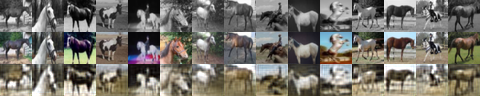
\includegraphics[width=10cm]{regression_output.png}
    \end{center}
    \item Using rgb color space can be problematic since it does not capture other attributes that are central to how human perceives color, such as lightness and saturation. 
    \item L2 regularization severely penalizes outliers, so will try to overfit the model to the dataset during training. If we frame colorization as a classification problem, then the loss function of each sample will not experience similar problem as when we frame colorization as a regression problem. 
\end{enumerate}


\textbf{B. Colorization as Classification}


\begin{enumerate}
    \item 
    \item The predicted images for model \texttt{CNN} have more saturated colors and in most cases matches with the original images when compared to \texttt{RegressionCNN}.
    \begin{center}
        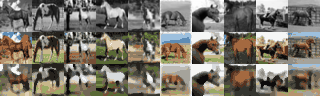
\includegraphics[width=10cm]{eval_CNN.png}
    \end{center}
\end{enumerate}


\textbf{C. Skip Connections}


\begin{enumerate}
    \item Training curve as follows
    \begin{center}
        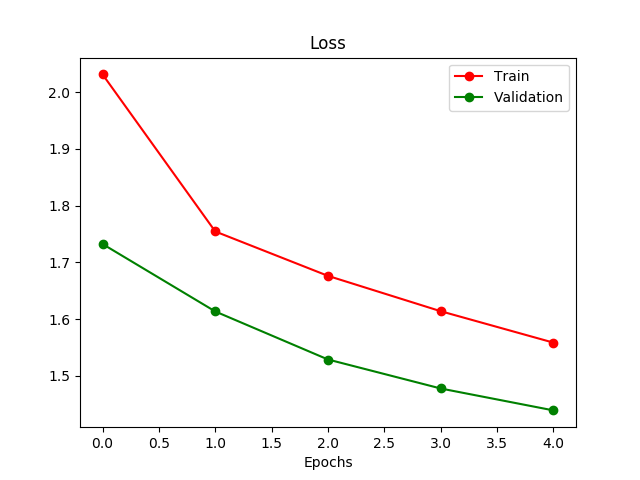
\includegraphics[width=10cm]{unet_training_curve.png}
    \end{center}
    \item The answer is based on the pretrained \texttt{UNet} model provided (25 epochs). As the table below have shown, the skip connection improve validation loss and accuracy. Qualitatively, the \texttt{UNet} generated slightly more accurate colorization than \texttt{CNN} as shown below.
    \begin{center}
        \begin{tabular}{c | c c}
            model & validation loss & validation accuracy \\
            \hline 
            \texttt{CNN} & 1.5881 & 41.1\%\\
            \texttt{UNet} & 1.3659 & 48.0\%\\
        \end{tabular}
    \end{center}
    \begin{enumerate}
        \item \texttt{CNN} \,\, 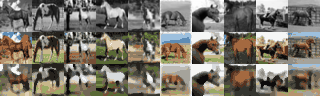
\includegraphics[width=10cm]{eval_CNN.png}
        \item \texttt{UNet} 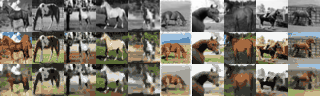
\includegraphics[width=10cm]{eval_UNet.png} 
    \end{enumerate}
    Here we give two reasons why skip connections might improve perfomance of \texttt{CNN} models 
    \begin{enumerate}
        \item Skip connection helps with supplying features to the latter layers in the convolutional neural network where certain features are lost due to upsampling
        \item Skip connection might make optimization more effective as it allows for backpropagation to adjust parameters early in the network. 
    \end{enumerate}
\end{enumerate}

\textbf{D. Dilated Convolution}


\begin{enumerate}
    \item Let $C_{in}$ be input channel size, $C_{out}$ be output channel size, and $k$ be kernel size. The weights and receptive field for different types of convolutions are shown below,
    \begin{center}
        \begin{tabular}{c | c c}
            filter & weights & receptive field (filter) size \\
            \hline 
            $3\times 3$ convolution & $9C_{in}C_{out}$ & $3\times 3$ \\
            $5\times 5$ convolution & $25C_{in}C_{out}$ & $5\times 5$ \\ 
            $3\times 3$ convolution with dilation 1 & $9C_{in}C_{out}$ & $5\times 5$ \\
        \end{tabular}
    \end{center}
    \item \texttt{DilatedUNet} replaces the middle convolution with a dilated convolution with dilation 1 here instead of another convolution because it is the layer that represents a turning point from max pooling to upsampling. Dilated convolution with dilation 1, by enlarging receptive field, will preserve the feature map size for purpose described. Additionally, dilated convolution integrate knowledge of a wider context in the input feature map by enlarging the receptive field.
\end{enumerate}


\textbf{E. Visualizing Intermediate Activations}

\begin{enumerate}
    \item The activations in first few layers preserve the contour, or shape of the input image approximately and the weights (color in greyscale) are typically similar in similar regions of the feature map. The activation in latter layers have weights (color in greyscale) that differ in the same region of the feature map. This implies that the output color channels in some region of the generated image are affected by one or a few input feature map. The later layers 
    \begin{center}
        \includegraphics[width=1cm]{act1_cnn/filter_input_1.png}
        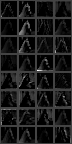
\includegraphics[width=2cm]{act1_cnn/filter_out0_1.png}
        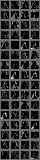
\includegraphics[width=2cm]{act1_cnn/filter_out1_1.png}
        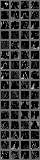
\includegraphics[width=2cm]{act1_cnn/filter_out2_1.png}
        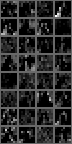
\includegraphics[width=2cm]{act1_cnn/filter_out3_1.png}
        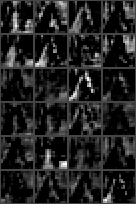
\includegraphics[width=2cm]{act1_cnn/filter_out4_1.png}
        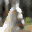
\includegraphics[width=1cm]{act1_cnn/filter_output_1.png}
        \includegraphics[width=1cm]{act1_cnn/filter_input_rgb_1.png}
    \end{center}
    \item We notice that the activations in layers (especially activations for the first and last convolution) for \texttt{UNet} resemble of a blend the corresponding layers in \texttt{CNN}. The earlier layers capture some color pattern and the latter layers exhibit inclusion of contour/shape pattern.
    \begin{center}
        \includegraphics[width=1cm]{act1_unet/filter_input_1.png}
        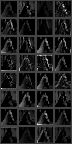
\includegraphics[width=2cm]{act1_unet/filter_out0_1.png}
        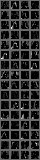
\includegraphics[width=2cm]{act1_unet/filter_out1_1.png}
        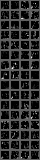
\includegraphics[width=2cm]{act1_unet/filter_out2_1.png}
        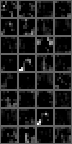
\includegraphics[width=2cm]{act1_unet/filter_out3_1.png}
        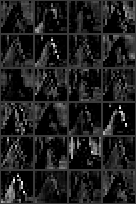
\includegraphics[width=2cm]{act1_unet/filter_out4_1.png}
        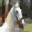
\includegraphics[width=1cm]{act1_unet/filter_output_1.png}
        \includegraphics[width=1cm]{act1_unet/filter_input_rgb_1.png}
    \end{center}
\end{enumerate}


\textbf{F. Conceptual Problems}

\begin{enumerate}
    \item Only b would be helpful in augmenting the data for our \texttt{CNN} model. The model would be exposed to a larger variety of cases where the subject of the image is a horse. Larger training dataset helps with generalization of the model and thus improve performance. Options like c and d would make the model overfit as max pooling makes model translation invariant. Option a would not be useful in this case, since an image flipped upside down does not describe realistic scenario. Option e would not be useful since the added image consists of subject other than horse, which we aim to color.
    \item A list of some hyperparameters 
    \begin{enumerate}
        \item number of filters (depth)
        \item stride
        \item padding
        \item convolution filter size (receptive field)
        \item pooling filter size (spatial extent)
        \item dilation 
    \end{enumerate}
\end{enumerate}

\textbf{G. Dilated Convolution Implementation}

\begin{enumerate}
    \item 
    \item Quantitatively, the \texttt{DUNet} model achieved worse validation loss and accuracy than \texttt{UNet} but better validation loss and accuracy than \texttt{CNN}. Qualitativey, \texttt{DUNet} performed similarly to \texttt{UNet}, although we observed there åre miss-colorizations in some regions of the predicted image. Dilated filters maybe more efficient in cases where there are consecutive convolution layers stacked together; The receptive field for dilated convolution layer grows faster without the added cost of trainable parameters.
    \begin{center} 
        \begin{tabular}{c | c c}
            model & validation loss & validation accuracy \\
            \hline 
            \texttt{CNN} & 1.5881 & 41.1\%\\
            \texttt{UNet} & 1.3659 & 48.0\%\\
            \texttt{DUNet} & 1.4353 & 45.8\%\\
        \end{tabular}
    \end{center}
    \begin{enumerate}
        \item \texttt{UNet} \,\,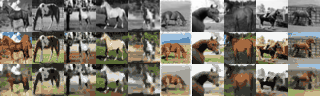
\includegraphics[width=10cm]{eval_UNet.png} 
        \item \texttt{DUNet} 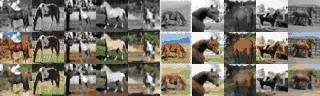
\includegraphics[width=10cm]{eval_DUNet.png} 
    \end{enumerate}
\end{enumerate}


\end{document}
